%
% spektralradius.tex
%
% (c) 2020 Prof Dr Andreas Müller, Hochschule Rapperswil
%
\begin{frame}[fragile]
\definecolor{darkgreen}{rgb}{0,0.6,0}
\definecolor{orange}{rgb}{1,0.4,0}
\def\polargrid{
\pgfmathparse{60*3.1/3.14159}
\xdef\winkel{\pgfmathresult}
\foreach \r in {-3,-2.7,...,3.1}{
	\draw[color=orange,line width=0.5pt] 
		({-3+3*exp(\r/3)*exp(-1)*cos(-\winkel)},{3*exp(\r/3)*exp(-1)*sin(-\winkel)})
		arc (-\winkel:\winkel:{3*exp(\r/3)*exp(-1)});
	\draw[color=darkgreen,line width=0.5pt]
		({-3+2.9*exp(-2)*cos(60*\r/3.14159)},{2.9*exp(-2)*sin(60*\r/3.14159)})
		--
		({-3+3.1*cos(60*\r/3.14159)},{3.1*sin(60*\r/3.14159)});
}

}
\def\rectangulargrid{
\foreach \y in {-3,-2.7,...,3.1}{
	\draw[color=darkgreen,line width=0.5pt] (-3.1,\y)--(3.1,\y);
	\draw[color=orange,line width=0.5pt] (\y,-3.1)--(\y,3.1);
}
}
\def\punkt#1#2{
	\fill[color=white] ({3*#1},{3*#2}) circle[radius=0.04];
	\draw[color=red] ({3*#1},{3*#2}) circle[radius=0.04];
}
\def\spektralradius#1{
	\fill[color=blue!20] (0,0) circle[radius={3*#1}];
	\draw[color=blue,line width=0.5pt] (0,0) circle[radius={3*#1}];
}
\def\achsen{
	\draw[->] (-3.1,0)--(3.3,0) coordinate[label={$\text{Re}$}];
	\draw[->] (0,-3.1)--(0,3.3) coordinate[label={right:$\text{Im}$}];
	\draw (-3,-0.1)--(-3,0.1); \node at (-3,-0.1) [below right] {$-1$};
	\draw (3,-0.1)--(3,0.1);   \node at (3,-0.1) [below right] {$1$};
	\draw (-0.1,3)--(0.1,3);   \node at (0,3) [below right] {$1$};
	\draw (-0.1,-3)--(0.1,-3);
	
}
\def\matrixA{
\spektralradius{0.9964}
\rectangulargrid
\punkt{0.7995}{0.4778}
\punkt{-0.3111}{-0.2504}
\punkt{-0.8832}{-0.0940}
\punkt{-0.2848}{-0.7000}
\punkt{0.0244}{-0.6006}
\punkt{0.0063}{-0.2695}
\punkt{0.3594}{-0.0205}
\punkt{-0.1645}{0.3118}
\punkt{0.7343}{0.4931}
\punkt{-0.6826}{0.6476}
\punkt{-0.8291}{0.0196}
\punkt{-0.4247}{-0.8782}
\punkt{-0.9964}{-0.0110}
\punkt{-0.1609}{0.4427}
\punkt{-0.8684}{0.2432}
\punkt{0.1513}{0.0202}
\punkt{-0.8265}{-0.1304}
\punkt{-0.5771}{0.2772}
\punkt{-0.2441}{-0.6865}
\punkt{-0.8256}{0.2559}
\punkt{-0.3171}{-0.3922}
\punkt{-0.1067}{0.4191}
\punkt{0.7999}{-0.4032}
\punkt{0.1777}{0.7223}
\punkt{-0.8979}{0.2560}
\punkt{-0.1108}{-0.9879}
\punkt{0.8914}{-0.2691}
\punkt{-0.6339}{-0.7629}
\punkt{-0.1702}{0.3504}
\punkt{0.7651}{0.1889}
\punkt{-0.1850}{-0.7487}
\punkt{0.2580}{0.5141}
\punkt{-0.3368}{0.5461}
\punkt{0.0477}{0.2592}
\punkt{-0.2233}{0.4031}
\punkt{-0.2602}{0.0218}
\punkt{0.7916}{-0.0305}
\punkt{-0.3862}{0.1043}
\punkt{-0.1751}{0.6592}
\punkt{0.1907}{-0.7383}
\punkt{0.0214}{-0.5192}
\punkt{-0.1587}{0.2889}
\punkt{0.0947}{0.6130}
\punkt{-0.6335}{-0.0430}
\punkt{0.0899}{-0.1559}
\punkt{-0.1458}{-0.8521}
\punkt{0.1713}{-0.5716}
\punkt{-0.0225}{0.8633}
\punkt{0.6110}{0.4059}
\punkt{-0.9506}{-0.2428}
\punkt{0.7995}{-0.4778}
\punkt{-0.3111}{0.2504}
\punkt{-0.8832}{0.0940}
\punkt{-0.2848}{0.7000}
\punkt{0.0244}{0.6006}
\punkt{0.0063}{0.2695}
\punkt{0.3594}{0.0205}
\punkt{-0.1645}{-0.3118}
\punkt{0.7343}{-0.4931}
\punkt{-0.6826}{-0.6476}
\punkt{-0.8291}{-0.0196}
\punkt{-0.4247}{0.8782}
\punkt{-0.9964}{0.0110}
\punkt{-0.1609}{-0.4427}
\punkt{-0.8684}{-0.2432}
\punkt{0.1513}{-0.0202}
\punkt{-0.8265}{0.1304}
\punkt{-0.5771}{-0.2772}
\punkt{-0.2441}{0.6865}
\punkt{-0.8256}{-0.2559}
\punkt{-0.3171}{0.3922}
\punkt{-0.1067}{-0.4191}
\punkt{0.7999}{0.4032}
\punkt{0.1777}{-0.7223}
\punkt{-0.8979}{-0.2560}
\punkt{-0.1108}{0.9879}
\punkt{0.8914}{0.2691}
\punkt{-0.6339}{0.7629}
\punkt{-0.1702}{-0.3504}
\punkt{0.7651}{-0.1889}
\punkt{-0.1850}{0.7487}
\punkt{0.2580}{-0.5141}
\punkt{-0.3368}{-0.5461}
\punkt{0.0477}{-0.2592}
\punkt{-0.2233}{-0.4031}
\punkt{-0.2602}{-0.0218}
\punkt{0.7916}{0.0305}
\punkt{-0.3862}{-0.1043}
\punkt{-0.1751}{-0.6592}
\punkt{0.1907}{0.7383}
\punkt{0.0214}{0.5192}
\punkt{-0.1587}{-0.2889}
\punkt{0.0947}{-0.6130}
\punkt{-0.6335}{0.0430}
\punkt{0.0899}{0.1559}
\punkt{-0.1458}{0.8521}
\punkt{0.1713}{0.5716}
\punkt{-0.0225}{-0.8633}
\punkt{0.6110}{-0.4059}
\punkt{-0.9506}{0.2428}
}
\def\richardson{
\spektralradius{0.8694}
\polargrid
\punkt{-0.1352}{-0.2385}
\punkt{-0.2733}{-0.3763}
\punkt{-0.2470}{-0.3212}
\punkt{-0.3247}{-0.3629}
\punkt{-0.1352}{0.2385}
\punkt{-0.2733}{0.3763}
\punkt{-0.2470}{0.3212}
\punkt{-0.1885}{-0.0248}
\punkt{-0.1885}{0.0248}
\punkt{-0.3247}{0.3629}
\punkt{-0.2234}{0.1485}
\punkt{-0.2234}{-0.1485}
\punkt{-0.3773}{-0.2676}
\punkt{-0.3773}{0.2676}
\punkt{-0.6708}{-0.2996}
\punkt{-0.6703}{-0.2905}
\punkt{-0.5854}{-0.2342}
\punkt{-0.4731}{-0.0108}
\punkt{-0.4731}{0.0108}
\punkt{-0.6708}{0.2996}
\punkt{-0.5854}{0.2342}
\punkt{-0.6703}{0.2905}
\punkt{-0.8188}{-0.2749}
\punkt{-0.8188}{0.2749}
\punkt{-0.7662}{-0.2734}
\punkt{-0.7662}{0.2734}
\punkt{-0.6328}{-0.2362}
\punkt{-0.6328}{0.2362}
\punkt{-0.6692}{-0.2327}
\punkt{-0.6692}{0.2327}
\punkt{-0.7906}{-0.2393}
\punkt{-0.8464}{-0.1852}
\punkt{-0.7906}{0.2393}
\punkt{-0.6890}{0.2130}
\punkt{-0.6890}{-0.2130}
\punkt{-0.8464}{0.1852}
\punkt{-0.5721}{-0.0086}
\punkt{-0.5721}{0.0086}
\punkt{-0.7760}{-0.2081}
\punkt{-0.6737}{-0.1865}
\punkt{-0.7760}{0.2081}
\punkt{-0.6737}{0.1865}
\punkt{-0.6024}{-0.0625}
\punkt{-0.7559}{-0.1891}
\punkt{-0.6024}{0.0625}
\punkt{-0.8589}{0.1349}
\punkt{-0.7771}{-0.1827}
\punkt{-0.8589}{-0.1349}
\punkt{-0.7559}{0.1891}
\punkt{-0.6270}{-0.0989}
\punkt{-0.7884}{0.1783}
\punkt{-0.7884}{-0.1783}
\punkt{-0.6270}{0.0989}
\punkt{-0.7771}{0.1827}
\punkt{-0.6431}{-0.0986}
\punkt{-0.6431}{0.0986}
\punkt{-0.8518}{-0.1121}
\punkt{-0.6980}{-0.1345}
\punkt{-0.8518}{0.1121}
\punkt{-0.7755}{-0.1364}
\punkt{-0.7170}{-0.1342}
\punkt{-0.6980}{0.1345}
\punkt{-0.7755}{0.1364}
\punkt{-0.7170}{0.1342}
\punkt{-0.6991}{-0.0894}
\punkt{-0.7086}{-0.1065}
\punkt{-0.7030}{-0.0957}
\punkt{-0.7293}{-0.1154}
\punkt{-0.7293}{0.1154}
\punkt{-0.7524}{0.1024}
\punkt{-0.6991}{0.0894}
\punkt{-0.7524}{-0.1024}
\punkt{-0.7030}{0.0957}
\punkt{-0.7086}{0.1065}
\punkt{-0.8013}{-0.0565}
\punkt{-0.7389}{-0.0668}
\punkt{-0.7389}{0.0668}
\punkt{-0.7165}{-0.0062}
\punkt{-0.8013}{0.0565}
\punkt{-0.8620}{-0.0342}
\punkt{-0.7513}{0.0260}
\punkt{-0.8550}{-0.0379}
\punkt{-0.8620}{0.0342}
\punkt{-0.7165}{0.0062}
\punkt{-0.8550}{0.0379}
\punkt{-0.8441}{-0.0408}
\punkt{-0.8642}{-0.0015}
\punkt{-0.8441}{0.0408}
\punkt{-0.8642}{0.0015}
\punkt{-0.8502}{0.0372}
\punkt{-0.8502}{-0.0372}
\punkt{-0.7513}{-0.0260}
\punkt{-0.8486}{0.0143}
\punkt{-0.8049}{-0.0084}
\punkt{-0.8404}{0.0209}
\punkt{-0.8486}{-0.0143}
\punkt{-0.8049}{0.0084}
\punkt{-0.8395}{0.0031}
\punkt{-0.8395}{-0.0031}
\punkt{-0.8404}{-0.0209}
}

\frametitle{Spektralradius}
\vspace{-25pt}
\begin{columns}[t]
\begin{column}{6.5cm}
\begin{center}
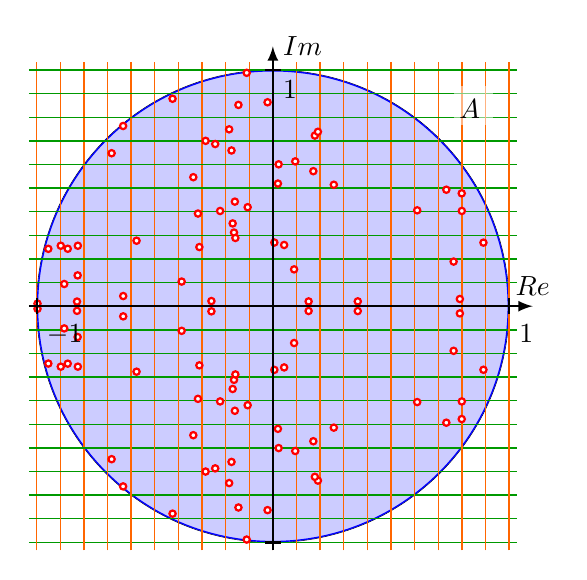
\begin{tikzpicture}[>=latex,thick]
\begin{scope}
\clip (-3.1,-3.1) rectangle (3.1,3.1);
\draw[line width=0.2pt] (0,0) circle[radius=3];
\matrixA
\fill[color=white,opacity=0.5] (2.3,2.3) rectangle (2.8,2.8);
\node at (2.5,2.5) {$A$};
\end{scope}
\achsen
\end{tikzpicture}
\end{center}
\end{column}
\begin{column}{6.5cm}
\begin{center}
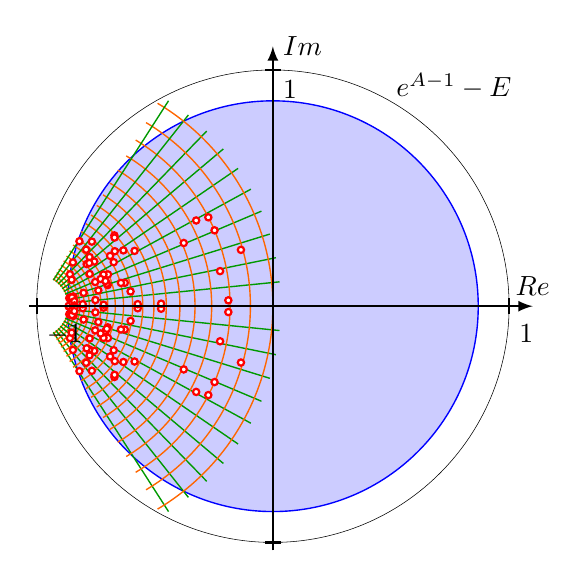
\begin{tikzpicture}[>=latex,thick]
\begin{scope}
\clip (-3.1,-3.1) rectangle (3.1,3.1);
\draw[line width=0.2pt] (0,0) circle[radius=3];
\uncover<2->{
\richardson
\node at (2.3,2.8) {$e^{A-1}-E$};
}
\end{scope}
\achsen
\end{tikzpicture}
\end{center}
\end{column}
\end{columns}
\end{frame}
